\documentclass[aspectratio=169, 10pt]{beamer}

% ==============================================================================
% Packages & Professional Academic Typography
% ==============================================================================
\usepackage[utf8]{inputenc}
\usepackage[T1]{fontenc}
\usepackage{lmodern}
\usepackage{microtype}
\usepackage{booktabs}
\usepackage{array}
\usepackage{amsmath,amssymb}
\usepackage[most]{tcolorbox}
\usepackage{tikz}
\usetikzlibrary{automata, positioning, arrows.meta, shapes.geometric, calc, fit}

% ==============================================================================
% Design System & Refined Academic Color Palette (GIMPA Branding)
% ==============================================================================
\definecolor{gimpanavy}{RGB}{10, 37, 64}       % #0A2540 Deep Academic Navy
\definecolor{gimpaslate}{RGB}{51, 65, 85}      % #334155 Slate Gray
\definecolor{gimpaaccent}{RGB}{30, 107, 184}   % #1E6BB8 Scholarly Blue
\definecolor{charcoalText}{RGB}{30, 41, 59}     % #1E293B High-contrast body
\definecolor{lightBg}{RGB}{248, 250, 252}      % #F8FAFC Clean card background
\definecolor{ruleGray}{RGB}{226, 232, 240}     % #E2E8F0 Subtle divider
\definecolor{accentCrimson}{RGB}{185, 28, 28}  % #B91C1C Academic Alert
\definecolor{accentGreen}{RGB}{21, 128, 61}    % #15803D Success / Verification
\definecolor{accentAmber}{RGB}{180, 83, 9}     % #B45309 Amber Warning / Key Insight

% Beamer General Settings
\setbeamertemplate{navigation symbols}{}
\setbeamercolor{background canvas}{bg=white}
\setbeamercolor{normal text}{fg=charcoalText}
\setbeamercolor{structure}{fg=gimpanavy}
\setbeamercolor{title}{fg=gimpanavy}
\setbeamercolor{author}{fg=gimpaslate}
\setbeamercolor{institute}{fg=gimpaslate}
\setbeamercolor{date}{fg=gimpaslate}

% Clean, Dignified Frametitle
\setbeamertemplate{frametitle}{
  \vspace{0.12cm}
  \noindent
  {\large\bfseries\color{gimpanavy}\insertframetitle}
  \ifx\insertframesubtitle\@empty\else
    \\[0.03cm]{\footnotesize\color{gimpaslate}\insertframesubtitle}
  \fi
  \vspace{0.04cm}
  {\color{ruleGray}\hrule height 0.6pt}
  \vspace{0.05cm}
}

% Sleek Minimalist Footline
\setbeamertemplate{footline}{
  \vspace{-0.40cm}
  \begin{center}
    {\color{ruleGray}\rule{0.95\paperwidth}{0.5pt}}
  \end{center}
  \vspace{-0.15cm}
  \leavevmode%
  \hbox{%
    \begin{beamercolorbox}[wd=0.45\paperwidth,ht=2.5ex,dp=1.2ex,left]{footline}%
      \hspace*{0.6cm}{\scriptsize\color{gimpaslate}\textbf{CS 305: Theory of Computation} \;\textbar\; Week 1}
    \end{beamercolorbox}%
    \begin{beamercolorbox}[wd=0.33\paperwidth,ht=2.5ex,dp=1.2ex,center]{footline}%
      {\scriptsize\color{gimpaslate}GIMPA School of Technology}
    \end{beamercolorbox}%
    \begin{beamercolorbox}[wd=0.22\paperwidth,ht=2.5ex,dp=1.2ex,right]{footline}%
      {\scriptsize\color{gimpaslate}\insertframenumber{} / \inserttotalframenumber}\hspace*{0.6cm}
    \end{beamercolorbox}%
  }%
  \vspace*{0.20cm}
}

% Minimalist Square Bullets
\setbeamertemplate{itemize item}{{\color{gimpaaccent}\scriptsize$\blacksquare$}}
\setbeamertemplate{itemize subitem}{{\color{gimpaslate}\tiny$\blacktriangleright$}}
\setbeamertemplate{enumerate item}{\textbf{\color{gimpanavy}\insertenumlabel.}}

% ==============================================================================
% Card Environments & Section Styling
% ==============================================================================
\newcommand{\colheader}[1]{%
  {\noindent\footnotesize\bfseries\color{gimpanavy}#1}%
  \vspace{0.02cm}%
  {\color{gimpanavy!30}\hrule height 0.5pt}%
  \vspace{0.05cm}%
}

\newcommand{\cardtitle}[1]{{\noindent\footnotesize\bfseries\color{gimpanavy}#1}\par\vspace{0.03cm}}
\newcommand{\alerttitle}[1]{{\noindent\footnotesize\bfseries\color{accentCrimson}#1}\par\vspace{0.03cm}}
\newcommand{\ambertitle}[1]{{\noindent\footnotesize\bfseries\color{accentAmber}#1}\par\vspace{0.03cm}}
\newcommand{\greentitle}[1]{{\noindent\footnotesize\bfseries\color{accentGreen}#1}\par\vspace{0.03cm}}

\tcbset{
  before=\vspace{1pt},
  after=\vspace{1pt},
  top=2.5pt,
  bottom=2.5pt,
  left=5pt,
  right=5pt,
  boxrule=0.5pt,
  arc=2pt,
  conceptcard/.style={
    enhanced,
    colback=lightBg,
    colframe=ruleGray,
    borderline west={2.5pt}{0pt}{gimpanavy}
  },
  examplecard/.style={
    enhanced,
    colback=lightBg,
    colframe=ruleGray,
    borderline west={2.5pt}{0pt}{accentGreen}
  },
  alertcard/.style={
    enhanced,
    colback=lightBg,
    colframe=ruleGray,
    borderline west={2.5pt}{0pt}{accentCrimson}
  },
  spotlightcard/.style={
    enhanced,
    colback=gimpaaccent!5,
    colframe=ruleGray,
    borderline west={2.5pt}{0pt}{gimpaaccent}
  },
  quizcard/.style={
    enhanced,
    colback=accentAmber!5,
    colframe=ruleGray,
    borderline west={2.5pt}{0pt}{accentAmber}
  }
}

% TikZ Automata Settings
\tikzset{
  every state/.style={
    draw=gimpanavy,
    thick,
    fill=white,
    minimum size=7.5mm,
    inner sep=1pt,
    font=\small\bfseries\color{gimpanavy}
  },
  initial text={},
  initial distance=5mm,
  every initial by arrow/.style={
    ->,
    >=stealth,
    thick,
    draw=gimpanavy
  },
  accepting/.style={
    double,
    double distance=1.5pt,
    thick,
    draw=gimpanavy
  },
  every edge/.style={
    ->,
    >=stealth,
    thick,
    draw=gimpanavy,
    font=\footnotesize
  }
}

% ==============================================================================
% Course & Presentation Metadata
% ==============================================================================
\title{\textbf{\LARGE Preliminaries, Formal Languages \& Computation Models}}
\subtitle{\vspace{0.12cm}\large Week 1: Mathematical Foundations, The Chomsky Hierarchy, and Modern AI}
\author{\textbf{School of Technology}}
\institute{Ghana Institute of Management and Public Administration (GIMPA)}
\date{Academic Year 2026/2027}

\begin{document}

% ------------------------------------------------------------------------------
% SLIDE 1: Title Slide
% ------------------------------------------------------------------------------
\begin{frame}[plain]
  \vspace{0.4cm}
  \begin{center}
    {\scriptsize\bfseries\color{gimpaaccent}CS 305: THEORY OF COMPUTATION --- WEEK 1 LECTURE}\\[0.22cm]
    {\LARGE\bfseries\color{gimpanavy}Preliminaries, Formal Languages \&\\[0.08cm] Models of Computation}\\[0.22cm]
    {\normalsize\color{gimpaslate}Mathematical Foundations, The Chomsky Hierarchy, and Modern AI Frontiers}\\[0.30cm]
    
    {\color{ruleGray}\rule{0.6\paperwidth}{0.6pt}}\\[0.30cm]
    
    {\small\bfseries\color{gimpanavy}School of Technology}\\[0.06cm]
    {\footnotesize\color{gimpaslate}Ghana Institute of Management and Public Administration (GIMPA)}\\[0.20cm]
    {\scriptsize\color{gimpaslate}Textbook Reference: Michael Sipser, \textit{Introduction to the Theory of Computation} (3rd Ed.), Chapter 0}
  \end{center}
\end{frame}

% ------------------------------------------------------------------------------
% SLIDE 2: Course Architecture: What is Theory of Computation?
% ------------------------------------------------------------------------------
\begin{frame}{Course Architecture: What is Theory of Computation?}
  \framesubtitle{From fundamental mathematical limits to modern algorithmic efficiency}
  
  \begin{columns}[T]
    \begin{column}{0.32\textwidth}
      \colheader{1. Automata Theory}
      \begin{tcolorbox}[conceptcard]
        \cardtitle{Finite \& Stack Machines}
        \begin{itemize}\setlength{\itemsep}{1.5pt}\scriptsize
          \item Memory-bounded computational models.
          \item Deterministic \& Nondeterministic Finite Automata (DFA/NFA).
          \item Context-Free Grammars \& Pushdown Automata (PDA).
          \item Applied in: Compilers, Regex, and Deep Packet Inspection.
        \end{itemize}
      \end{tcolorbox}
    \end{column}
    
    \begin{column}{0.32\textwidth}
      \colheader{2. Computability Theory}
      \begin{tcolorbox}[conceptcard]
        \cardtitle{1930s -- 1950s: Solvability}
        \begin{itemize}\setlength{\itemsep}{1.5pt}\scriptsize
          \item What is computable in principle?
          \item Turing Machines (Alan Turing, 1936).
          \item The Church--Turing Thesis.
          \item Undecidability \& Halting Problem ($A_{\text{TM}}$).
          \item Limits of static program verification (Rice's Theorem).
        \end{itemize}
      \end{tcolorbox}
    \end{column}
    
    \begin{column}{0.32\textwidth}
      \colheader{3. Complexity Theory}
      \begin{tcolorbox}[conceptcard]
        \cardtitle{1960s -- Present: Efficiency}
        \begin{itemize}\setlength{\itemsep}{1.5pt}\scriptsize
          \item What is computable in practice?
          \item Asymptotic Time \& Space complexity bounds.
          \item Classes $\mathbf{P}$, $\mathbf{NP}$, and $\mathbf{NP}$-Complete.
          \item Cook--Levin Theorem \& 3SAT.
          \item Modern Cryptography, SAT solvers, and Quantum ($\mathbf{BQP}$).
        \end{itemize}
      \end{tcolorbox}
    \end{column}
  \end{columns}
  
  \vspace{0.10cm}
  \begin{tcolorbox}[spotlightcard]
    {\footnotesize\textbf{Central Question:} What are the fundamental capabilities and limitations of digital computers, and how does mathematical theory guide modern software systems?}
  \end{tcolorbox}
\end{frame}

% ------------------------------------------------------------------------------
% SLIDE 3: Course Mechanics & Expectations
% ------------------------------------------------------------------------------
\begin{frame}{Course Mechanics \& Evaluation Criteria}
  \framesubtitle{Pedagogical structure, grading breakdown, and learning expectations}
  
  \begin{columns}[T]
    \begin{column}{0.48\textwidth}
      \colheader{Course Structure \& Assessment}
      \begin{tcolorbox}[conceptcard]
        \cardtitle{Grading Distribution}
        \begin{itemize}\setlength{\itemsep}{2pt}\scriptsize
          \item \textbf{Problem Sets (4 Assignments, 25\%):} Rigorous mathematical proofs and automata design.
          \item \textbf{Quizzes \& Checks (2 Quizzes, 15\%):} In-class conceptual checkpoints.
          \item \textbf{Midterm Examination (20\%):} Automata, Regular Languages \& CFLs.
          \item \textbf{Term Project (15\%):} Hands-on automata simulator or formal verification tool.
          \item \textbf{Final Examination (25\%):} Comprehensive assessment.
        \end{itemize}
      \end{tcolorbox}
    \end{column}
    
    \begin{column}{0.48\textwidth}
      \colheader{Primary Literature \& Standards}
      \begin{tcolorbox}[conceptcard]
        \cardtitle{Required Textbook}
        {\scriptsize
        Michael Sipser, \textit{Introduction to the Theory of Computation}, 3rd International Edition, Cengage Learning.
        }
        \vspace{0.06cm}
        
        \cardtitle{Academic Expectations}
        \begin{itemize}\setlength{\itemsep}{2pt}\scriptsize
          \item \textbf{Mathematical Rigor:} Exact definitions, precise notation, and formal proofs.
          \item \textbf{Collaboration Policy:} Discussion encouraged; all proofs and code written individually.
        \end{itemize}
      \end{tcolorbox}
    \end{column}
  \end{columns}
  
  \vspace{0.10cm}
  \begin{tcolorbox}[quizcard]
    {\scriptsize\textbf{Diagnostic Prerequisite:} This course assumes familiarity with discrete mathematics: set theory, relations, functions, graphs, and proof by induction/contradiction. Review Sipser Chapter 0 this week.}
  \end{tcolorbox}
\end{frame}

% ------------------------------------------------------------------------------
% SLIDE 4: Why Theory Matters in 2026
% ------------------------------------------------------------------------------
\begin{frame}{Why Theory of Computation in 2026?}
  \framesubtitle{Theoretical boundaries govern everyday production engineering}
  
  \begin{columns}[T]
    \begin{column}{0.48\textwidth}
      \colheader{Everyday Systems Engineered on Theory}
      \begin{tcolorbox}[conceptcard]
        \cardtitle{Compilers \& Lexical Analyzers}
        {\scriptsize
        Lexers (Flex, LLVM) convert source code to tokens in guaranteed $\mathcal{O}(n)$ time by compiling regex to DFAs.
        }
        \vspace{0.06cm}
        
        \cardtitle{Network Firewalls (Zeek / Snort)}
        {\scriptsize
        Deep Packet Inspection engines scan gigabit-per-second traffic in real-time using parallel finite state machines.
        }
      \end{tcolorbox}
    \end{column}
    
    \begin{column}{0.48\textwidth}
      \colheader{Modern Frontiers: AI, Security \& Blockchain}
      \begin{tcolorbox}[spotlightcard]
        \cardtitle{Large Language Models (LLMs)}
        {\scriptsize
        Grammar-guided decoding (Outlines/Guidance) forces LLM logits through CFG state machines to guarantee valid JSON/SQL.
        }
        \vspace{0.06cm}
        
        \cardtitle{Smart Contract Gas (Ethereum)}
        {\scriptsize
        Because the Halting Problem is undecidable, blockchains cannot statically check termination; they charge ``Gas'' per step.
        }
      \end{tcolorbox}
    \end{column}
  \end{columns}
  
  \vspace{0.10cm}
  \begin{tcolorbox}[alertcard]
    {\scriptsize\textbf{Engineering Takeaway:} Theory is not abstract detachment; it is the ultimate architectural tool that tells engineers what is mathematically possible, what is intractable, and what is strictly impossible.}
  \end{tcolorbox}
\end{frame}

% ------------------------------------------------------------------------------
% SLIDE 5: Mathematical Foundations: Alphabets
% ------------------------------------------------------------------------------
\begin{frame}{Mathematical Foundations: Alphabets ($\Sigma$)}
  \framesubtitle{The atomic building blocks of all formal languages}
  
  \begin{columns}[T]
    \begin{column}{0.48\textwidth}
      \colheader{Formal Definition}
      \begin{tcolorbox}[conceptcard]
        \cardtitle{Definition 1.1: Alphabet}
        {\scriptsize
        An \textbf{alphabet} $\Sigma$ is a non-empty, \textbf{finite set} of symbols.
        }
        \vspace{0.06cm}
        
        \cardtitle{Critical Mathematical Requirements:}
        \begin{itemize}\setlength{\itemsep}{2pt}\scriptsize
          \item $\Sigma \ne \emptyset$ (Must contain at least one symbol).
          \item $|\Sigma| < \infty$ (Must be finite; infinite alphabets are excluded in standard automata theory).
          \item Symbols are atomic primitives.
        \end{itemize}
      \end{tcolorbox}
    \end{column}
    
    \begin{column}{0.48\textwidth}
      \colheader{Standard Computing Alphabets}
      \begin{tcolorbox}[examplecard]
        \greentitle{Ubiquitous Computing Examples:}
        \begin{itemize}\setlength{\itemsep}{2.5pt}\scriptsize
          \item \textbf{Binary Alphabet:} $\Sigma = \{0, 1\}$ (Digital circuits, assembly).
          \item \textbf{Decimal Alphabet:} $\Sigma_{10} = \{0, 1, 2, \dots, 9\}$.
          \item \textbf{English Alphabet:} $\Sigma_{\text{ENG}} = \{a, b, c, \dots, z\}$.
          \item \textbf{DNA Genetic Alphabet:} $\Sigma_{\text{DNA}} = \{A, C, G, T\}$.
          \item \textbf{ASCII Byte Alphabet:} $\Sigma_{256} = \{0x00, \dots, 0xFF\}$.
        \end{itemize}
      \end{tcolorbox}
    \end{column}
  \end{columns}
  
  \vspace{0.10cm}
  \begin{tcolorbox}[alertcard]
    {\scriptsize\textbf{Common Student Mistake:} An alphabet $\Sigma$ is a set of \textit{symbols}, NOT a set of strings. For example, $\{00, 11\}$ is a language over $\{0,1\}$, not an atomic alphabet.}
  \end{tcolorbox}
\end{frame}

% ------------------------------------------------------------------------------
% SLIDE 6: Strings and Words
% ------------------------------------------------------------------------------
\begin{frame}{Strings (Words) Over an Alphabet}
  \framesubtitle{Finite sequences formed from alphabet symbols}
  
  \begin{columns}[T]
    \begin{column}{0.48\textwidth}
      \colheader{Formal Definitions}
      \begin{tcolorbox}[conceptcard]
        \cardtitle{Definition 1.2: String (Word)}
        {\scriptsize
        A \textbf{string} $w$ over alphabet $\Sigma$ is a \textbf{finite sequence} of symbols from $\Sigma$:
        \[ w = w_1 w_2 \dots w_n \quad (w_i \in \Sigma) \]
        }
        \vspace{0.03cm}
        
        \cardtitle{String Length ($|w|$)}
        {\scriptsize
        The number of symbols in $w$. If $w = 10110$, $|w| = 5$.
        }
        \vspace{0.03cm}
        
        \cardtitle{The Empty String ($\varepsilon$ or $\lambda$)}
        {\scriptsize
        The unique string containing zero symbols: $|\varepsilon| = 0$.
        }
      \end{tcolorbox}
    \end{column}
    
    \begin{column}{0.48\textwidth}
      \colheader{String Concatenation \& Algebra}
      \begin{tcolorbox}[examplecard]
        \greentitle{Concatenation ($u \cdot v$ or $uv$)}
        {\scriptsize
        If $u = a_1 \dots a_m$ and $v = b_1 \dots b_n$, then:
        \[ uv = a_1 \dots a_m b_1 \dots b_n \]
        }
        \vspace{0.03cm}
        
        \greentitle{Algebraic Laws:}
        \begin{itemize}\setlength{\itemsep}{2pt}\scriptsize
          \item \textbf{Length Additivity:} $|uv| = |u| + |v|$.
          \item \textbf{Identity Element:} $\varepsilon u = u \varepsilon = u$.
          \item \textbf{Associativity:} $(uv)w = u(vw)$.
          \item \textbf{Non-Commutative:} In general, $uv \ne vu$ ($01 \ne 10$).
        \end{itemize}
      \end{tcolorbox}
    \end{column}
  \end{columns}
  
  \vspace{0.08cm}
  \begin{tcolorbox}[conceptcard]
    {\scriptsize\textbf{Algebraic Insight:} The set of strings over $\Sigma$ with concatenation form a \textbf{monoid} with identity element $\varepsilon$.}
  \end{tcolorbox}
\end{frame}

% ------------------------------------------------------------------------------
% SLIDE 7: String Operations: Powers, Reversal, Substrings
% ------------------------------------------------------------------------------
\begin{frame}{String Operations: Powers, Reversal, Substrings}
  \framesubtitle{Essential mathematical operations utilized throughout automata proofs}
  
  \begin{columns}[T]
    \begin{column}{0.32\textwidth}
      \colheader{String Powers ($w^k$)}
      \begin{tcolorbox}[conceptcard]
        \cardtitle{Inductive Definition}
        {\scriptsize
        \begin{align*}
          w^0 &= \varepsilon \\
          w^{k} &= w^{k-1} w \quad (k \ge 1)
        \end{align*}
        \textbf{Examples:}
        \begin{itemize}\setlength{\itemsep}{1.5pt}\scriptsize
          \item $(01)^3 = 010101$
          \item $a^4 = aaaa$
          \item $(11)^0 = \varepsilon$
        \end{itemize}
        }
      \end{tcolorbox}
    \end{column}
    
    \begin{column}{0.32\textwidth}
      \colheader{String Reversal ($w^R$)}
      \begin{tcolorbox}[examplecard]
        \greentitle{Inversion of Symbols}
        {\scriptsize
        If $w = w_1 w_2 \dots w_n$:
        \[ w^R = w_n \dots w_2 w_1 \]
        \textbf{Key Inversion Law:}
        \[ (uv)^R = v^R u^R \]
        \textbf{Palindrome Definition:}
        $w$ is a palindrome iff $w = w^R$.
        }
      \end{tcolorbox}
    \end{column}
    
    \begin{column}{0.32\textwidth}
      \colheader{Substrings \& Factors}
      \begin{tcolorbox}[spotlightcard]
        \cardtitle{Prefix, Suffix, Substring}
        {\scriptsize
        Let $w$ be a string:
        \begin{itemize}\setlength{\itemsep}{1.5pt}\scriptsize
          \item \textbf{Prefix:} $x$ where $w = xy$.
          \item \textbf{Suffix:} $y$ where $w = xy$.
          \item \textbf{Substring:} $y$ where $w = xyz$.
        \end{itemize}
        \textit{Note: $\varepsilon$ is a prefix, suffix, and substring of every string.}
        }
      \end{tcolorbox}
    \end{column}
  \end{columns}
  
  \vspace{0.10cm}
  \begin{tcolorbox}[alertcard]
    {\scriptsize\textbf{Proof Technique Tip:} Proving $(uv)^R = v^R u^R$ is done by induction on $|v|$. Notice how string concatenation reverses order, identical to matrix transposition $(AB)^T = B^T A^T$!}
  \end{tcolorbox}
\end{frame}

% ------------------------------------------------------------------------------
% SLIDE 8: Formal Languages Over an Alphabet
% ------------------------------------------------------------------------------
\begin{frame}{Formal Languages Over an Alphabet}
  \framesubtitle{A language is a set of strings: framing computation as decision problems}
  
  \begin{columns}[T]
    \begin{column}{0.48\textwidth}
      \colheader{Kleene Star \& The String Universe}
      \begin{tcolorbox}[conceptcard]
        \cardtitle{The Kleene Star ($\Sigma^*$)}
        {\scriptsize
        The set of \textbf{all finite strings} over $\Sigma$, including $\varepsilon$:
        \[ \Sigma^* = \bigcup_{k=0}^{\infty} \Sigma^k = \{\varepsilon, 0, 1, 00, 01, 10, 11, \dots\} \]
        }
        \vspace{0.03cm}
        
        \cardtitle{Kleene Plus ($\Sigma^+$)}
        {\scriptsize
        All strings except the empty string:
        \[ \Sigma^+ = \Sigma^* \setminus \{\varepsilon\} \]
        }
      \end{tcolorbox}
    \end{column}
    
    \begin{column}{0.48\textwidth}
      \colheader{Formal Definition of a Language}
      \begin{tcolorbox}[examplecard]
        \greentitle{Definition 1.3: Formal Language}
        {\scriptsize
        A \textbf{language} $L$ over alphabet $\Sigma$ is any subset of $\Sigma^*$:
        \[ L \subseteq \Sigma^* \]
        }
        \vspace{0.03cm}
        
        \greentitle{Examples over $\Sigma = \{0, 1\}$:}
        \begin{itemize}\setlength{\itemsep}{1.5pt}\scriptsize
          \item $L_1 = \{w \mid w \text{ contains substring } 11\}$
          \item $L_2 = \{w \mid w \text{ has an even number of } 0\text{s}\}$
          \item $L_3 = \{0^n 1^n \mid n \ge 0\} = \{\varepsilon, 01, 0011, \dots\}$
          \item $L_{\text{prime}} = \{1^p \mid p \text{ is prime}\}$
        \end{itemize}
      \end{tcolorbox}
    \end{column}
  \end{columns}
  
  \vspace{0.10cm}
  \begin{tcolorbox}[alertcard]
    {\scriptsize\textbf{Critical Distinction:} $\emptyset$ vs. $\{\varepsilon\}$ vs. $\varepsilon$. 
    $\emptyset$ is the \textbf{empty language} ($|\emptyset| = 0$ strings). 
    $\{\varepsilon\}$ is a \textbf{language containing 1 string} ($|\{\varepsilon\}| = 1$). 
    $\varepsilon$ is a \textbf{string} (not a set). Never confuse $\emptyset$ and $\{\varepsilon\}$!}
  \end{tcolorbox}
\end{frame}

% ------------------------------------------------------------------------------
% SLIDE 9: Check-in Quiz 1.1: Foundations Drill
% ------------------------------------------------------------------------------
\begin{frame}{In-Class Check-in 1.1: Mathematical Foundations}
  \framesubtitle{Test your conceptual understanding of alphabets, strings, and languages}
  
  \begin{columns}[T]
    \begin{column}{0.48\textwidth}
      \colheader{Conceptual Questions}
      \begin{tcolorbox}[quizcard]
        \ambertitle{Check-in Problem 1.1A}
        {\scriptsize
        Let $\Sigma = \{a, b\}$. 
        \begin{enumerate}\setlength{\itemsep}{2pt}\scriptsize
          \item What is $|\Sigma^3|$?
          \item Is $\emptyset \subseteq \Sigma^*$?
          \item Is $\varepsilon \in \emptyset$?
          \item Is $\varepsilon \in \Sigma^*$ ?
        \end{enumerate}
        }
        \vspace{0.06cm}
        
        \ambertitle{Check-in Problem 1.1B}
        {\scriptsize
        True or False: If language $L$ is infinite, must the underlying alphabet $\Sigma$ be infinite?
        }
      \end{tcolorbox}
    \end{column}
    
    \begin{column}{0.48\textwidth}
      \colheader{In-Class Workspace \& Discussion}
      \begin{tcolorbox}[conceptcard]
        \cardtitle{Student Analysis Prompts:}
        \begin{itemize}\setlength{\itemsep}{3pt}\scriptsize
          \item \textbf{Cartesian Power Rule:} How does $|\Sigma^k|$ scale with alphabet size $|\Sigma|$ and word length $k$?
          \item \textbf{Set-Theoretic Distinction:} Recall the strict difference between the \textit{empty set} $\emptyset$ (containing zero strings) and the \textit{empty string} $\varepsilon$ (containing zero symbols).
          \item \textbf{Countability Principle:} Review Sipser Section 0.2 on countably infinite languages $\Sigma^*$ constructed over finite alphabets $\Sigma$.
          \item \textbf{Collaborative Action:} Discuss your deductions with your peer before open class review.
        \end{itemize}
        \vspace{0.20cm}
        {\tiny\color{charcoalText}\textit{[Active learning drill --- solutions analyzed interactively in lecture.]}}
      \end{tcolorbox}
    \end{column}
  \end{columns}
  
  \vspace{0.10cm}
  \begin{tcolorbox}[spotlightcard]
    {\scriptsize\textbf{Pedagogical Key:} Every computational decision problem can be formalized as a \textbf{language decision problem}: ``Given string $w \in \Sigma^*$, is $w \in L$?''}
  \end{tcolorbox}
\end{frame}

% ------------------------------------------------------------------------------
% SLIDE 10: Modern AI Connection: LLM Tokenization Alphabets
% ------------------------------------------------------------------------------
\begin{frame}{Modern AI Connection: LLM Tokenization Alphabets}
  \framesubtitle{Byte-Pair Encoding (BPE) and why token alphabets break character reasoning}
  
  \begin{columns}[T]
    \begin{column}{0.50\textwidth}
      \colheader{Subword Tokenization (BPE)}
      \begin{tcolorbox}[conceptcard]
        \cardtitle{The Token Vocabulary Alphabet ($\Sigma_V$)}
        {\scriptsize
        LLMs define an alphabet of subword tokens:
        \[ \Sigma_V = \{0, 1, 2, \dots, |V|-1\} \]
        where $|V| \approx 32{,}000$ to $128{,}000$ unique tokens.
        \vspace{0.03cm}
        
        \textbf{Tokenization Mapping:}
        \[ \text{tokenize}: \Sigma_{\text{UTF8}}^* \to \Sigma_V^* \]
        \textbf{Example (cl100k\_base):}\par
        $\text{``strawberry''} \;\longrightarrow\; [\text{``str''}, \text{``aw''}, \text{``berry''}]$\par
        $= [4999, 1378, 19233]$ ($3$ symbols in $\Sigma_V^*$).
        }
      \end{tcolorbox}
    \end{column}
    
    \begin{column}{0.46\textwidth}
      \colheader{The ``How Many r's?'' Mystery}
      \begin{tcolorbox}[alertcard]
        \alerttitle{Why LLMs Fail Character Counts}
        {\scriptsize
        \textbf{Observation:} When asked \textit{``How many 'r's in strawberry?''}, unassisted LLMs often say 2 instead of 3.
        \vspace{0.03cm}
        
        \textbf{Theoretical Cause:}
        \begin{itemize}\setlength{\itemsep}{1pt}\scriptsize
          \item Input sequence is 3 tokens long.
          \item The letter \texttt{'r'} is NOT an atomic symbol in $\Sigma_V$.
          \item Model must recall spelling from dense vector weights without string inspection.
        \end{itemize}
        }
      \end{tcolorbox}
    \end{column}
  \end{columns}
  
  \vspace{0.04cm}
  \begin{tcolorbox}[spotlightcard]
    {\scriptsize\textbf{Formal Language Lesson:} The choice of alphabet $\Sigma$ determines the expressivity and difficulty of all downstream computational tasks.}
  \end{tcolorbox}
\end{frame}

% ------------------------------------------------------------------------------
% SLIDE 11: The Chomsky Hierarchy: Overview
% ------------------------------------------------------------------------------
\begin{frame}{The Chomsky Hierarchy: 4 Classes of Expressivity}
  \framesubtitle{Noam Chomsky (1956): Classifying grammars and their computational automata}
  
  \vspace{-0.1cm}
  \begin{center}
    \scriptsize
    \setlength{\tabcolsep}{3pt}
    \renewcommand{\arraystretch}{1.15}
    \begin{tabular}{@{} l l l l l @{}}
      \toprule
      \textbf{Type} & \textbf{Language Class} & \textbf{Recognizing Machine} & \textbf{Memory Model} & \textbf{Production Rules ($A \to \alpha$)} \\
      \midrule
      \textbf{Type 3} & \textbf{Regular} & Finite Automata (DFA/NFA) & $\mathcal{O}(1)$ Constant Memory & $A \to aB$ or $A \to a$ \\
      \textbf{Type 2} & \textbf{Context-Free} & Pushdown Automata (PDA) & LIFO Stack Memory & $A \to \gamma$ ($A \in V$) \\
      \textbf{Type 1} & \textbf{Context-Sensitive} & Linear Bounded Automata (LBA) & $\mathcal{O}(n)$ Bounded Tape & $\alpha A \beta \to \alpha \gamma \beta$ \\
      \textbf{Type 0} & \textbf{Turing-Recognizable} & Turing Machine (TM) & $\mathcal{O}(\infty)$ Unbounded Tape & $\alpha \to \beta$ (Unrestricted) \\
      \bottomrule
    \end{tabular}
  \end{center}
  
  \vspace{-0.1cm}
  \begin{columns}[T]
    \begin{column}{0.48\textwidth}
      \begin{tcolorbox}[conceptcard]
        \cardtitle{Strict Subset Hierarchy}
        {\scriptsize
        \[ \mathcal{L}_3 \subsetneq \mathcal{L}_2 \subsetneq \mathcal{L}_1 \subsetneq \mathcal{L}_0 \]
        Every regular language is context-free, but CFLs describe nested recursive syntax beyond finite automata.
        }
      \end{tcolorbox}
    \end{column}
    
    \begin{column}{0.48\textwidth}
      \begin{tcolorbox}[spotlightcard]
        \cardtitle{Why Memory Dictates Power}
        {\scriptsize
        The progression from Type 3 to Type 0 is an evolution of \textbf{storage}:
        No memory $\longrightarrow$ Stack $\longrightarrow$ Linear tape $\longrightarrow$ Infinite tape.
        }
      \end{tcolorbox}
    \end{column}
  \end{columns}
\end{frame}

% ------------------------------------------------------------------------------
% SLIDE 12: TikZ Visual: The Concentric Hierarchy
% ------------------------------------------------------------------------------
\begin{frame}{Visualizing the Expressive Hierarchy}
  \framesubtitle{Concentric containment of formal language classes and automata models}
  
  \vspace{-0.05cm}
  \begin{center}
    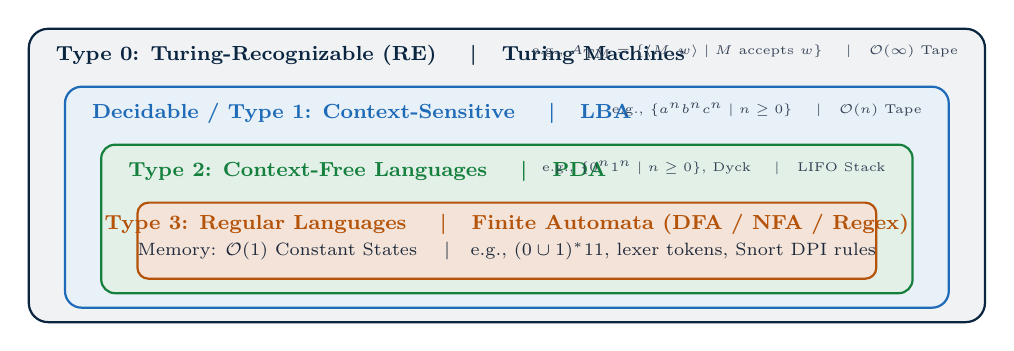
\begin{tikzpicture}[scale=0.92, every node/.style={transform shape}]
      % Type 0
      \draw[rounded corners=7pt, thick, fill=gimpanavy!6, draw=gimpanavy] (-6.6, -2.0) rectangle (6.6, 2.05);
      \node[anchor=north west] at (-6.35, 1.95) {\footnotesize\bfseries\color{gimpanavy}Type 0: Turing-Recognizable (RE) \quad\textbar\quad Turing Machines};
      \node[anchor=north east] at (6.35, 1.95) {\tiny\color{gimpaslate}e.g., $A_{\text{TM}} = \{\langle M, w \rangle \mid M \text{ accepts } w\}$ \quad\textbar\quad $\mathcal{O}(\infty)$ Tape};

      % Type 1 / Decidable
      \draw[rounded corners=6pt, thick, fill=gimpaaccent!10, draw=gimpaaccent] (-6.1, -1.8) rectangle (6.1, 1.25);
      \node[anchor=north west] at (-5.85, 1.15) {\footnotesize\bfseries\color{gimpaaccent}Decidable / Type 1: Context-Sensitive \quad\textbar\quad LBA};
      \node[anchor=north east] at (5.85, 1.15) {\tiny\color{gimpaslate}e.g., $\{a^n b^n c^n \mid n \ge 0\}$ \quad\textbar\quad $\mathcal{O}(n)$ Tape};

      % Type 2
      \draw[rounded corners=5pt, thick, fill=accentGreen!12, draw=accentGreen] (-5.6, -1.6) rectangle (5.6, 0.45);
      \node[anchor=north west] at (-5.35, 0.35) {\footnotesize\bfseries\color{accentGreen}Type 2: Context-Free Languages \quad\textbar\quad PDA};
      \node[anchor=north east] at (5.35, 0.35) {\tiny\color{gimpaslate}e.g., $\{0^n 1^n \mid n \ge 0\}$, Dyck \quad\textbar\quad LIFO Stack};

      % Type 3
      \draw[rounded corners=4pt, thick, fill=accentAmber!16, draw=accentAmber] (-5.1, -1.4) rectangle (5.1, -0.35);
      \node at (0, -0.65) {\footnotesize\bfseries\color{accentAmber}Type 3: Regular Languages \quad\textbar\quad Finite Automata (DFA / NFA / Regex)};
      \node at (0, -1.02) {\scriptsize\color{charcoalText}Memory: $\mathcal{O}(1)$ Constant States \quad\textbar\quad e.g., $(0 \cup 1)^* 11$, lexer tokens, Snort DPI rules};
    \end{tikzpicture}
  \end{center}
  
  \vspace{-0.15cm}
  \begin{tcolorbox}[conceptcard]
    {\scriptsize\textbf{Course Trajectory:} Over the next 14 weeks, we climb this hierarchy from inside out: Weeks 1--5 (Regular) $\longrightarrow$ Weeks 6--8 (Context-Free) $\longrightarrow$ Weeks 9--12 (Turing-Recognizable \& Undecidable) $\longrightarrow$ Weeks 13--15 (Complexity).}
  \end{tcolorbox}
\end{frame}

% ------------------------------------------------------------------------------
% SLIDE 13: Research Spotlight: Neural Networks & Chomsky (ICLR 2023)
% ------------------------------------------------------------------------------
\begin{frame}{Research Spotlight: Neural Networks \& The Chomsky Hierarchy}
  \framesubtitle{G.~Delétang et al. (Google DeepMind), ICLR 2023 Spotlight Paper}
  
  \begin{columns}[T]
    \begin{column}{0.48\textwidth}
      \colheader{The Research Question}
      \begin{tcolorbox}[spotlightcard]
        \cardtitle{Where do Deep Learning Models Lie?}
        {\scriptsize
        Deep neural networks achieve human-like fluencies, but \textbf{what is their theoretical computational capacity} on formal languages?
        
        DeepMind tested architectures across Chomsky levels:
        \begin{itemize}\setlength{\itemsep}{1.5pt}\scriptsize
          \item Feedforward Networks (MLP)
          \item Recurrent Networks (RNN, LSTM)
          \item Standard Transformers (Self-Attention)
          \item Neural Networks augmented with Stack / Tape Memory
        \end{itemize}
        }
      \end{tcolorbox}
    \end{column}
    
    \begin{column}{0.48\textwidth}
      \colheader{DeepMind's Empirical Findings}
      \begin{tcolorbox}[alertcard]
        \alerttitle{Key Theoretical Limits:}
        \begin{itemize}\setlength{\itemsep}{2pt}\scriptsize
          \item \textbf{Transformers $\approx$ Regular / Weak CFL:} Fixed-depth Transformers fail to generalize on deeply nested parentheses (Dyck languages) when input length exceeds training window.
          \item \textbf{Recurrent Models (LSTM) $\approx$ Counter Machines:} Can count one counter ($a^n b^n$), but fail at multiple nested dependencies.
          \item \textbf{External Memory is Strictly Required:} Neural models achieve Type 2 only with explicit stack, and Type 0 only with read/write tape.
        \end{itemize}
      \end{tcolorbox}
    \end{column}
  \end{columns}
  
  \vspace{0.08cm}
  \begin{tcolorbox}[conceptcard]
    {\scriptsize\textbf{Takeaway for AI Practitioners:} Without external scratchpads (Chain-of-Thought) or tool calling, Transformer LLMs are strictly memory-bounded and cannot solve arbitrary algorithmic reasoning!}
  \end{tcolorbox}
\end{frame}

% ------------------------------------------------------------------------------
% SLIDE 14: Introduction to Automata: The Intuition of Finite Control
% ------------------------------------------------------------------------------
\begin{frame}{Introduction to Automata: The Intuition of Finite Control}
  \framesubtitle{Abstract machines with finite internal states and no external storage}
  
  \begin{columns}[T]
    \begin{column}{0.50\textwidth}
      \colheader{Real-World Paradigm: The Automatic Door}
      \begin{tcolorbox}[conceptcard]
        \cardtitle{System Specifications}
        {\scriptsize
        An automatic sliding door at a store entrance:
        \begin{itemize}\setlength{\itemsep}{1.5pt}\scriptsize
          \item \textbf{Two States:} \texttt{CLOSED}, \texttt{OPEN}.
          \item \textbf{Alphabet of Sensor Inputs:}
          \begin{itemize}\setlength{\itemsep}{1pt}\scriptsize
            \item \texttt{FRONT}: Person on front mat.
            \item \texttt{REAR}: Person on rear mat.
            \item \texttt{BOTH}: People on both mats.
            \item \texttt{NEITHER}: No persons detected.
          \end{itemize}
        \end{itemize}
        }
      \end{tcolorbox}
    \end{column}
    
    \begin{column}{0.46\textwidth}
      \colheader{State Transition Graph}
      \begin{center}
        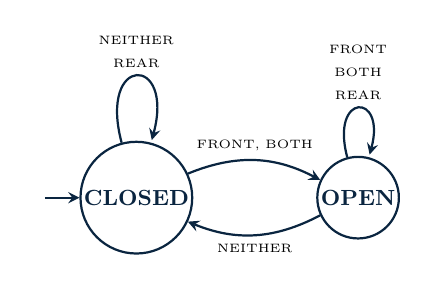
\begin{tikzpicture}[scale=0.88, every node/.style={transform shape}]
          \node[state, initial] (closed) at (0, 0) {\small CLOSED};
          \node[state] (open) at (3.2, 0) {\small OPEN};
          
          \path (closed) edge[loop above] node[align=center]{\tiny NEITHER\\\tiny REAR} (closed)
                (closed) edge[bend left=25] node[above]{\tiny FRONT, BOTH} (open)
                (open)   edge[loop above] node[align=center]{\tiny FRONT\\\tiny BOTH\\\tiny REAR} (open)
                (open)   edge[bend left=25] node[below]{\tiny NEITHER} (closed);
        \end{tikzpicture}
      \end{center}
    \end{column}
  \end{columns}
  
  \vspace{0.08cm}
  \begin{tcolorbox}[examplecard]
    {\scriptsize\textbf{Core Intuition of Finite Automata:} The machine has \textbf{no separate RAM or memory tape}. Its entire history of past inputs is compressed into its \textbf{current state}. This makes finite automata extremely fast ($\mathcal{O}(1)$ transition time) but fundamentally limited in counting.}
  \end{tcolorbox}
\end{frame}

% ------------------------------------------------------------------------------
% SLIDE 15: Preview of Week 2: Deterministic Finite Automata (DFA)
% ------------------------------------------------------------------------------
\begin{frame}{Preview of Week 2: Deterministic Finite Automata}
  \framesubtitle{Moving from informal diagrams to the rigorous 5-tuple mathematical definition}
  
  \begin{columns}[T]
    \begin{column}{0.48\textwidth}
      \colheader{The Formal 5-Tuple Definition}
      \begin{tcolorbox}[conceptcard]
        \cardtitle{Definition 1.4: DFA (Preview)}
        {\scriptsize
        A Deterministic Finite Automaton $M$ is a 5-tuple:
        \[ M = (Q, \Sigma, \delta, q_0, F) \]
        \begin{itemize}\setlength{\itemsep}{1.5pt}\scriptsize
          \item $Q$: Finite set of states.
          \item $\Sigma$: Finite input alphabet.
          \item $\delta: Q \times \Sigma \to Q$: Transition function.
          \item $q_0 \in Q$: Initial (start) state.
          \item $F \subseteq Q$: Set of accept (final) states.
        \end{itemize}
        }
      \end{tcolorbox}
    \end{column}
    
    \begin{column}{0.48\textwidth}
      \colheader{Example: Substring ``11'' Recognizer}
      \begin{center}
        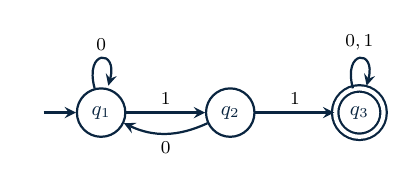
\begin{tikzpicture}[scale=0.82, every node/.style={transform shape}]
          \node[state, initial] (q1) at (0, 0) {$q_1$};
          \node[state] (q2) at (2.0, 0) {$q_2$};
          \node[state, accepting] (q3) at (4.0, 0) {$q_3$};
          
          \path (q1) edge[loop above] node{$0$} (q1)
                (q1) edge node[above]{$1$} (q2)
                (q2) edge[bend left=25] node[below]{$0$} (q1)
                (q2) edge node[above]{$1$} (q3)
                (q3) edge[loop above] node{$0, 1$} (q3);
        \end{tikzpicture}
      \end{center}
      \begin{tcolorbox}[examplecard]
        \greentitle{Language Recognized:}
        {\scriptsize
        \[ L(M) = \{w \in \{0, 1\}^* \mid w \text{ contains substring } 11\} \]
        Accepts: \texttt{01101}, \texttt{11}. Rejects: \texttt{01010}, \texttt{101}.
        }
      \end{tcolorbox}
    \end{column}
  \end{columns}
  
  \vspace{0.08cm}
  \begin{tcolorbox}[spotlightcard]
    {\scriptsize\textbf{Coming Up in Week 2:} Formal execution traces, state transition tables, closure properties (Union/Intersection via Cartesian Product construction), and line-rate Deep Packet Inspection in Zeek/Snort.}
  \end{tcolorbox}
\end{frame}

% ------------------------------------------------------------------------------
% SLIDE 16: Week 1 Synthesis & Diagnostic Math Review
% ------------------------------------------------------------------------------
\begin{frame}{Week 1 Synthesis \& Action Items}
  \framesubtitle{Summary of foundations and preparation for Week 2}
  
  \begin{columns}[T]
    \begin{column}{0.48\textwidth}
      \colheader{Week 1 Concept Checklist}
      \begin{tcolorbox}[conceptcard]
        \cardtitle{You should now be able to:}
        \begin{itemize}\setlength{\itemsep}{2pt}\scriptsize
          \item Define alphabet $\Sigma$, string $w$, and language $L \subseteq \Sigma^*$.
          \item Compute string powers $w^k$, reversals $w^R$, and understand length additivity $|uv| = |u| + |v|$.
          \item Differentiate rigorously between $\emptyset$, $\{\varepsilon\}$, and $\varepsilon$.
          \item Articulate the 4 levels of the Chomsky Hierarchy and how memory dictates expressive power.
          \item Explain the connection between LLM subword tokenization and character reasoning limits.
        \end{itemize}
      \end{tcolorbox}
    \end{column}
    
    \begin{column}{0.48\textwidth}
      \colheader{Readings \& Diagnostic Assignment}
      \begin{tcolorbox}[examplecard]
        \greentitle{Required Readings}
        \begin{itemize}\setlength{\itemsep}{1.5pt}\scriptsize
          \item Sipser (3rd Ed.), \textbf{Chapter 0: Introduction} (pp.~1--28).
          \item Sipser (3rd Ed.), \textbf{Section 1.1: Finite Automata} (pp.~31--44).
          \item Delétang et al., \textit{``Neural Networks and the Chomsky Hierarchy,''} ICLR 2023 (Spotlight).
        \end{itemize}
        \vspace{0.04cm}
        
        \greentitle{Action Items}
        \begin{itemize}\setlength{\itemsep}{1.5pt}\scriptsize
          \item Complete \textbf{Diagnostic Math Review} (Problem Set 0).
          \item Practice proving statements using induction and contradiction.
          \item Next Class: \textbf{DFA Formal 5-Tuples \& State Diagram Design}.
        \end{itemize}
      \end{tcolorbox}
    \end{column}
  \end{columns}
  
  \vspace{0.08cm}
  \begin{tcolorbox}[spotlightcard]
    \centering
    {\scriptsize\textbf{Questions?} Office Hours: Tuesdays \& Thursdays 14:00--16:00 GMT \;\textbar\; GIMPA School of Technology}
  \end{tcolorbox}
\end{frame}

\end{document}
